\documentclass[eng,printmode]{mgr}
\usepackage{listings}
\usepackage[english, polish]{babel}
\usepackage{graphicx}
\usepackage{hyperref}
\usepackage{tabularx,colortbl} 
\usepackage{rotating}
\usepackage{polski}
\usepackage[utf8]{inputenc} 
\setlength\parindent{24pt}
\usepackage[parfill]{parskip}
\usepackage{listings}
\usepackage[table,kernelfbox,hyperref]{xcolor}
\usepackage[xindy]{glossaries}
\usepackage{fancyhdr}
\usepackage{amsmath}
\usepackage{subfig}
\usepackage{float}

%\usepackage[colorinlistoftodos]{todonotes}

\hypersetup{colorlinks=true}
\hypersetup{xurlbordercolor=red!70!black}
\hypersetup{xlinkbordercolor=blue!70!black}
\hypersetup{linkcolor=blue!60!black}
\hypersetup{urlcolor=red!50!black}
\hypersetup{citecolor=green!30!black}
\makeglossaries
\rfoot{Page \thepage}
\renewcommand\lstlistlistingname{List of Listings}
\newcommand{\linia}{\rule{\linewidth}{0.4mm}}

\definecolor{listlightgray}{gray}{0.93}

\newcommand{\lstsetmylst} {
	\lstset{frame = tb,
		breaklines=true,
		framerule = 0.25pt,
		float,
		fontadjust,
		backgroundcolor={\color{listlightgray}},
		basicstyle = {\ttfamily\footnotesize},
		identifierstyle = {\ttfamily},
		stringstyle = {\ttfamily},
		showstringspaces = false,
		showtabs = false,
		numbers = left,
		numbersep = 6pt,
		tabsize = 4,
		language=C,
		floatplacement=!h
	}
}

\newcommand{\lstsetatc} {
	\lstset{frame = tb,
		breaklines=true,
		framerule = 0.25pt,
		float,
		fontadjust,
		backgroundcolor={\color{listlightgray}},
		basicstyle = {\ttfamily\footnotesize},
		keywordstyle = {\ttfamily\color{listkeyword}\textbf},
		identifierstyle = {\ttfamily},
		commentstyle = {\ttfamily\color{listcomment}\textit},
		stringstyle = {\ttfamily},
		showstringspaces = false,
		showtabs = false,
		numbers = left,
		numbersep = 6pt,
		numberstyle={\ttfamily\color{listnumbers}},
		tabsize = 4,
		language=C,
		floatplacement=!h
	}
}

\newcommand{\lstsetatbashnum} {
	\lstset{frame = tb,
		breaklines=true,
		framerule = 0.25pt,
		aboveskip=2ex,
		float,
		fontadjust,
		backgroundcolor={\color{listlightgray}},
		basicstyle = {\ttfamily\footnotesize},
		keywordstyle = {\ttfamily\color{listkeyword}\textbf},
		identifierstyle = {\ttfamily},
		commentstyle = {\ttfamily\color{listcomment}\textit},
		stringstyle = {\ttfamily},
		showstringspaces = false,
		showtabs = false,
		numbers = left,
		numbersep = 6pt,
		numberstyle={\ttfamily\color{listnumbers}},
		tabsize = 4,
		language=bash,
		floatplacement=!h
	}
}
\author{Jarosław Szumega, B.Sc.}
\title{}
\engtitle{}
\supervisor{Paweł Kabacik, D.Sc., \\ Onboard Telecommunication Electronics for Spacecraft and Transportation Means,\\Chair of Acoustics and Multimedia (W4/K-5),\\Wroclaw University of Science and Technology}
\field{Electronics Engineering}
\specialisation{Advanced Applied Electronics}
\date{2018}
\begin{document}
	%\pagestyle{fancy}

	\selectlanguage{english}
	\maketitle
	\frontmatter
	\tableofcontents
	\addcontentsline{toc}{chapter}{Contents}
	%\listoffigures
	\addcontentsline{toc}{chapter}{List of Figures}
	\lstsetmylst
	\mainmatter
\chapter{Introductory tasks}
\section{Problem statement}
The goal of the first task was to perform basic calculations and answer question related to principal knowledge in the area of microwave engineering.\\
The first task is to calculate the delution level of milk in the Baltic sea in decibels, while the second one is to answer how the complex impedance can be matched in microwave circuits.
\section{Tasks realization}
{\normalsize a1) One liter of milk diluted in the Baltic sea -- how many dB does it mean?}
\begin{align*}
V_{milk} &= 1\, liter\, = 1\, dm^3 = 10^{-3}\, m^3 \\
\\
V_{Baltic} &= 21\, 700\, km^3 = 21\, 700 \cdot 10^9\, m^3 =\\ 
		   &= 2.17\, \cdot 10^{13}\, m^3 \\
		   \\
Ratio_{dB} &= 10\, log_{10}\left(\frac{V_{milk}}{V_{Baltic}}\right) = \\
		   &= 10\, log_{10}\left(\frac{10^{-3}\, m^3}{2.17\, \cdot 10^{13}\, m^3}\right) = \\
		   &= -163.22\, dB
\end{align*}
{\normalsize a2) One liter of milk diluted in the Atlantic ocean -- how many dB does it mean?}
\begin{align*}
Ratio_{dB} &= 10\, log_{10}\left(\frac{V_{milk}}{V_{Atlantic}}\right) = 10\, log_{10}\left(\frac{10^{-3}\, m^3}{3.10\, \cdot 10^{17}\, m^3}\right)) =-204,91\, dB
\end{align*}
{\normalsize a3) Calculate volume of milk diluted in Atlantic ocean that is expressed as -225 dB.}
\begin{align*}
V_{milk} &= 10^{(\frac{db_value}{10})}\cdot V_{Atlantic} = 10^{(\frac{-225}{10})} \cdot 3.1 \cdot 10^{17}  = 9.8 \cdot 10^{-6}m^{3}= 9.8 * 10^{-3} litres
\end{align*}
\newpage
{\normalsize b) How to match the complex impedance?}

\begin{figure}[h]
	\centering
	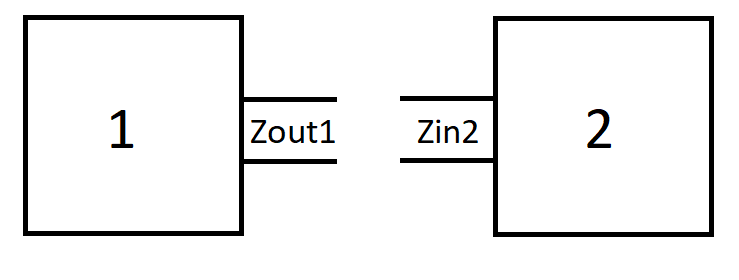
\includegraphics[width=0.3\linewidth]{matching}
	\label{fig:matching}
\end{figure}
\noindent
Q: What should be the relation between $Z_{out1}$ and $Z_{in2}$, so the impedances are "matched"?
\\
\\
A: The one of the numbers should be equal to complex conjugate of tother one, as presented in the equation below.
\begin{align*}
Z_{out1}\, &= \, {Z_{in2}}^*
\end{align*}
\\
The complex conjugate ($Z^*$) of given complex number $Z$ is defined in the following way:
\begin{align*}
Z &= x + j\cdot y \\
Z^* &= x - j\cdot y \\
\end{align*}
\section{Summary}
The introductory tasks covered basic, but essential aspects of microwave engineering. Expressing the ratio of powers or intensities in decibels is a common way to present these dependencies and matching impedances in the circuits is a common step in electrical equipment design.\\
As of the essential conclusions -- the second task was to find the relation between impedances in terms on matching them. As it was presented, to match two impedances, one should be a complex conjugate of the another.

\chapter{Basics of Microwave Engineering}
\section{Problem statement}
The assignment is to collect and present the information about microstrip, stripline and waveguides usage in the microwave engineering.\\
These three aproaches differ among themselves, have their advantages and disadvantages -- detailed review of these aspects will be presented.
\section{Task realization}
Waveguides and transmission lines are both elements designed to be interconnects between receivers and transmitters of the EM waves (to be more precise -- in range of radio frequencies and microwaves). Despite having similar role, there are essential differences among their properties.

\begin{figure}[h]
	\centering
	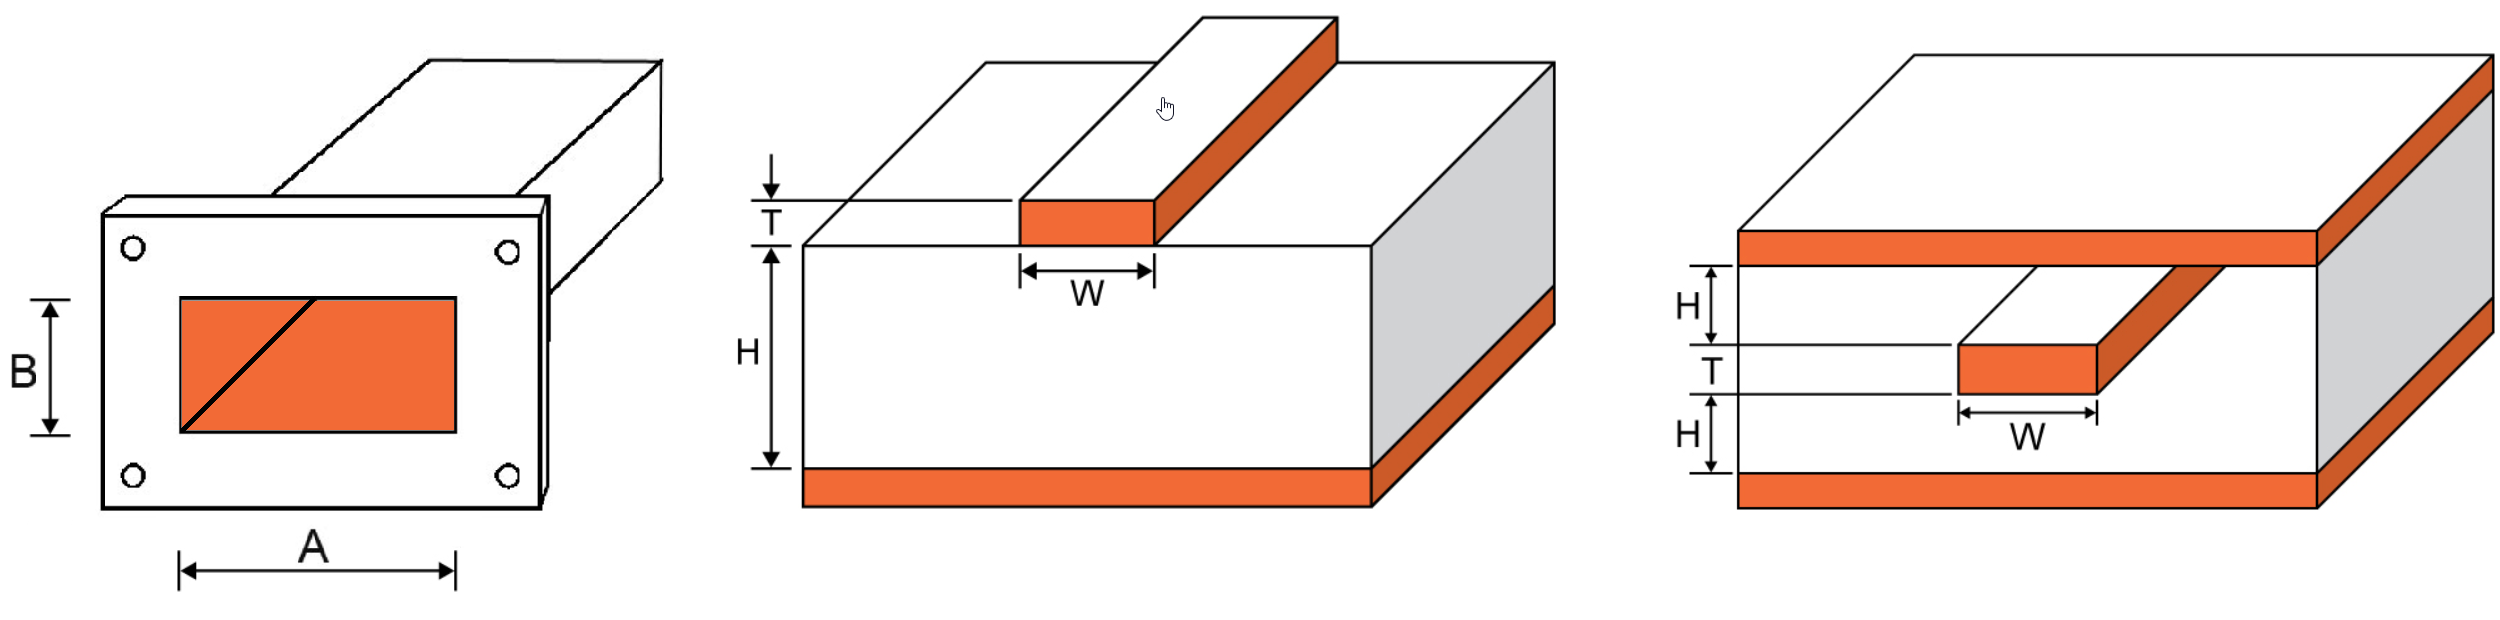
\includegraphics[width=0.8\linewidth]{technology}
	\caption{From left: waveguide, microstrip and stripline} (image source: https://www.allaboutcircuits.com)
	\label{fig:technology}
\end{figure}

	
%\subsubsection{Waveguides review \footnote{Waveguide Primer -- Introduction, article in resource \cite{microwave}.}}

\subsubsection{Waveguides review }
The waveguide is manufactured out of one conductor (in opposite to printed lines, what will be cleared in next paragraph). It is said, that waveguide has certain advantages over the printed lines
%\footnote{Waveguide Primer -- Introduction \cite{microwave}.}
%\footnote{Ibidem.}
-- due to its shielding, it can provide the isolation between adjacent signals. In addition, it is capable to transmit high peak powers, while having negligible losses in range of microwave frequencies.\\
It is also worth mentioning, that all kind of waveguide components are available (circulators, isolators, attenuators, loads, mixers, amplifiers).
\\
On the other hand, there still remain the disadvantages such as small manufactured volumes coming with high prices of waveguides materials (copper and silver). Also the dimensions and weight of waveguide are significant. Because of above--mentioned single conductor, the waveguide cannot provide a transverse-electromagnetic mode of transmission.

\subsubsection{Printed lines review}
%\subsubsection{Printed lines review \footnote{Transmission lines -- Microstrip and Stripline, article in resource \cite{microwave}.}}
Transmission lines used in printed circuits boards manufacturing are microstrips and striplines.\\
The stripline is a conductor placed between a dielectric pair of ground planes ("sandwiched"). It is a TEM (Transverse Electro--Magnetic) transmission line, what means it is non--dispersive. It is one of stripline's advantage over the microstrips. Also, the isolation between adjacent traces can be achieved.\\
One of the disadvantages of stripline is its complexity in fabrication, what also makes it more expensive than microstrip. The second one is a result of the second ground plane. The strip widths shall be narrower for a given impedance and board thickness than microstrips. 
An example to illustrate, for replacing N mils thick microstrips, the stripline should be 4N mils thick.
\\
\\
The microstrip transmission lines is a conductive strip of certain dimensions (width and thickness) with the wider ground plane. They are separated by a dielectric layer called "substrate" (also characterized by another thickness dimensions). \\According to the "Microwave Encyclopedia", microstrips are the most popular transmission lines especially for MIMICs (Monolithic Microwave Integrated Circuits).
Its advantage over stripline is that all active components can be mounted on top of the boards. However, for filtering, they may be required to provide external shielding of the circuit. In addition to disadvantages, the microstrip circuits can radiate and are dispersive (signals of different frequencies travel with different speeds). The TEM mode is not supported.

\section{Summary}
%As the three families of microwave components were introduced, it is essential to distinguish and sum--up their main features.\\
The waveguides are able to transmit high peak powers with very low losses in microwaves frequencies. Unfortunately, they are expensive and heavy equipment.\\
The striplines (conductor sandwiched between dielectric) are non--dispersive transmission lines supported TEM modes. They are more expensive than microstrip and more complex in fabrication.\\
The microstrips are at the moment very commonly used because of the ease of fabrication and usage. Unfortunately, they do not support TEM modes, often require external shielding and the circuit radiation has to be taken into consideration during the design process.

\newpage
\chapter{Microstrip vs stripline -- loss calculation using PCAAD}
\section{Problem statement}
During the class, there were given sets of parameters such as laminate and paths thickness, frequency, dielectric constant and impedance.\\The goal of the following task was to calculate total loss given in [dB/cm].\\
When the calculations are finished, the results shall be compared to total loss of the waveguides.
\\
\section{Task realization}
To perform the calculation, the PCAAD software version 7.0 was used ( PCAAD -- Personal Computer Aided Antenna Design).
\begin{figure}[h]
	\centering
	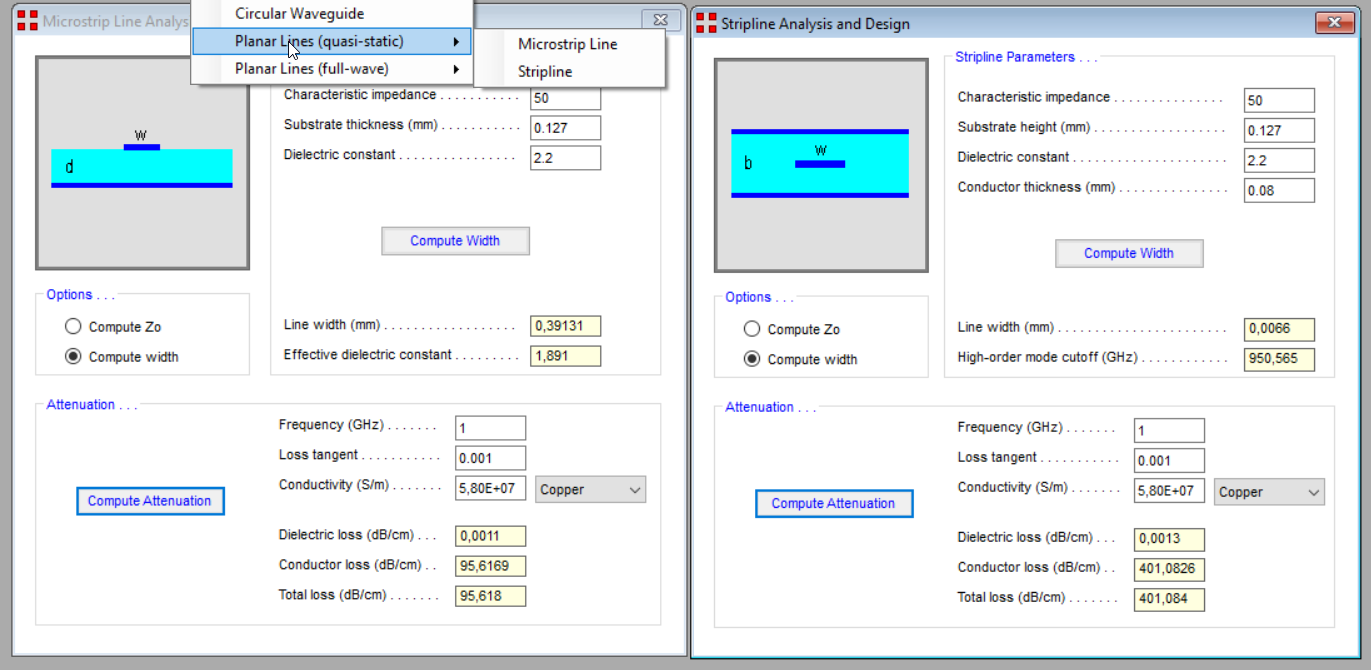
\includegraphics[width=0.7\linewidth]{pcaad}
	\caption{The quasi static methods interface for planar lines calculations}
	(screenshot taken during the usage of PCAAD v7.0)
	\label{fig:pcaad}
\end{figure}

\newpage
\begin{table}[h]
	\centering
	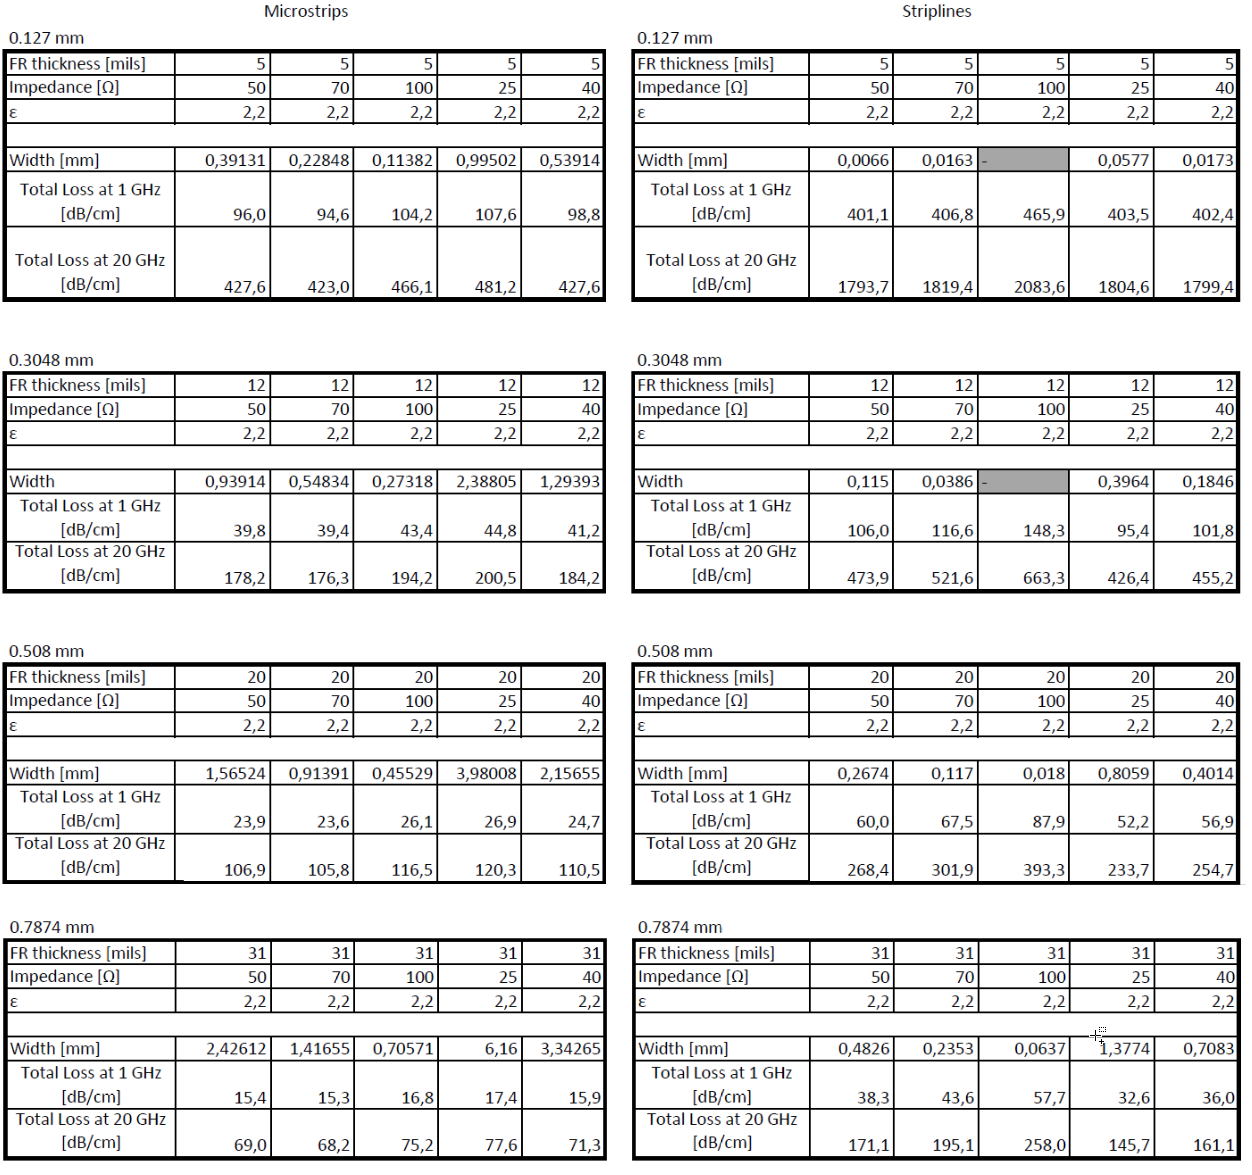
\includegraphics[width=1\linewidth]{table1a}
	\label{fig:microm1}
	\caption{The calculations made for listed parameters, $\epsilon$ = 2.2 and conductor thickness = 0.080mm (80 $\mu$m). Most of the results are calculated correctly, however there are examples where PCAAD software failed to give a results. They are marked with gray color.}
\end{table}

\begin{figure}[H]
\noindent
The results from the first striplines table show quite a significant total losses (~400 dB/cm for 1GHz and almost 1800-2000 db/cm for 20 GHz).
At the very beginning it was considered a mistake, but after retrying, the results were simply the same:
\\

	\centering{
	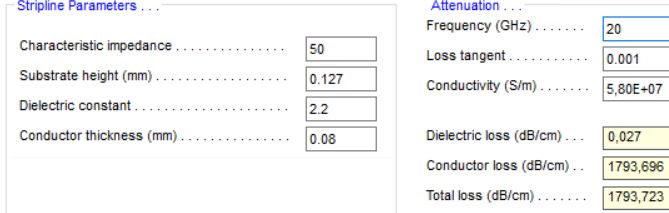
\includegraphics[width=0.7\linewidth]{pcaad2}}
	\label{fig:pcaad2}
	\caption{Recalculated example of stripline -- it was necessary to be sure, that the high value of loss is not a mistake.}
\end{figure}


\begin{table}[h]
	\centering
	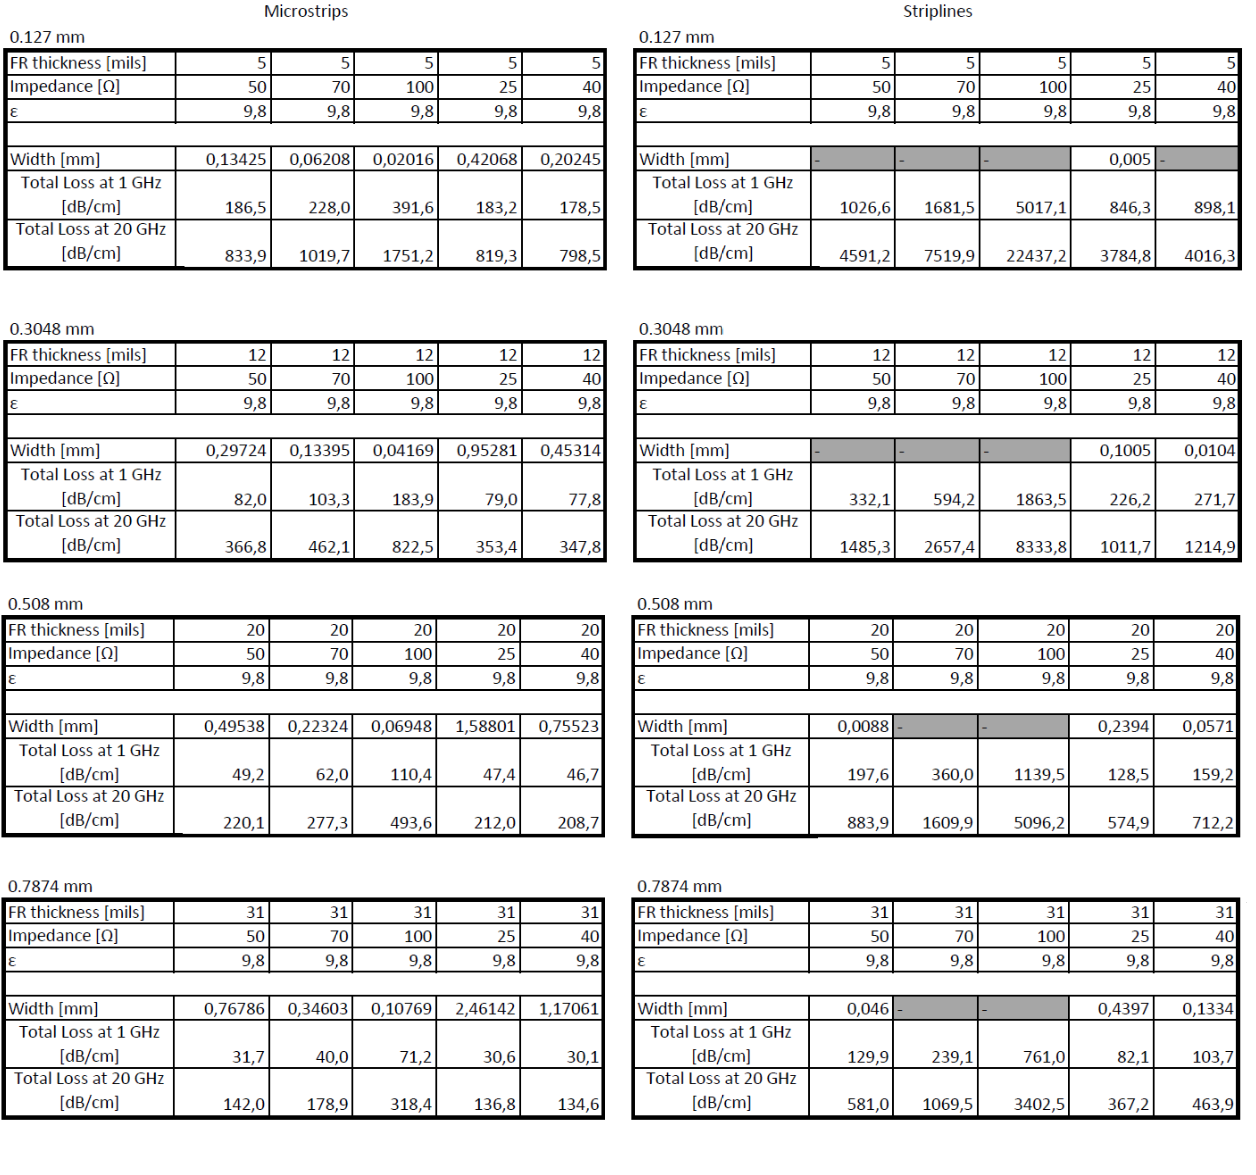
\includegraphics[width=1\linewidth]{table2a}
	\label{fig:microm2}
	\caption{The calculations made for $\epsilon$ = 9.8 and conductor thickness = 0.080mm (80 $\mu$m). It can be observed, that change of the epsilon from 2.2 to 9.8 causes significant increasing of the total losses. There is also more cases, where the width couldn't be calculated.}
\end{table}

Some calculations (cells marked with gray color) were plain wrong either due to obtaining negative values of width or recevining \textbf{Nan} result (NaN means "Not a Number" in floating point representation).\\
Professor's piece of advice during the lab was to compare quasi--static analysis with full--wave. Also in case if this approach fails, it was recommended to try a different tool for calculations:
\begin{itemize}
	\item the PCAAD v7.0 full--wave calculations fails, because the path width is a part of input data, so it cannot be calculated.
	\item website \textbf{Microwave101} also failed to calculate the missing values. The example will be presented below.
	\item open--source tools found on different websites failed mostly due the fact, that they allow to calculate the input impedance, not the total losses.
\end{itemize}

\begin{figure}
	\centering
	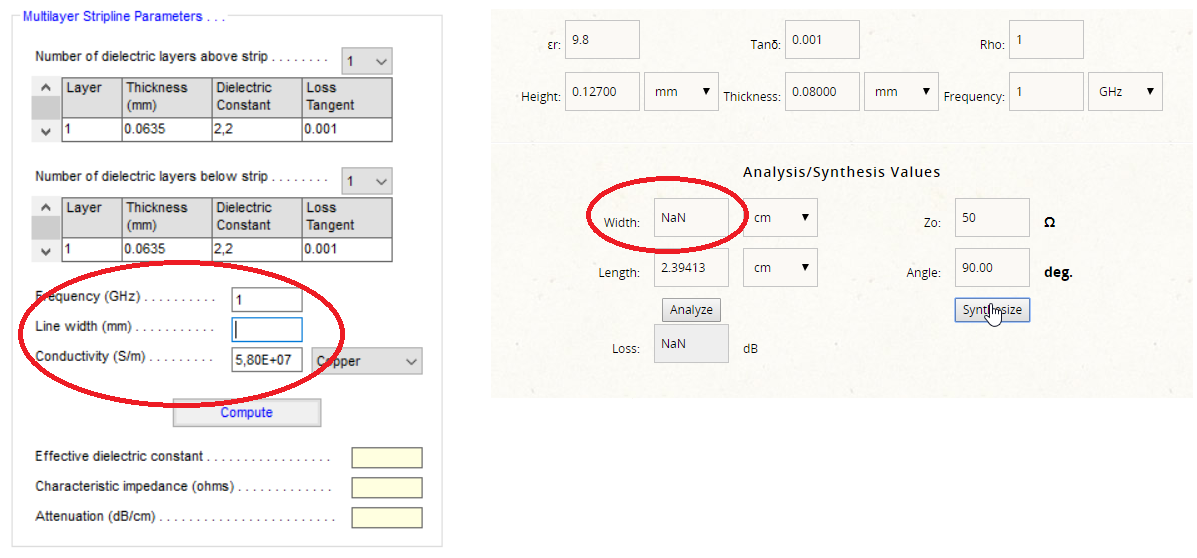
\includegraphics[width=0.7\linewidth]{microwave-fail}
	\caption{PCAAD v7.0 full-wave analysis (left image) and Microwave101 calculator (right) failed to improve missing. PCAAD's full--wave is not capable of width calculation as it is input data. Microwave101 also responds with "Not a Number" result.}
	\label{fig:microwave-fail}
\end{figure}
The assignment's second part was to compare the calculated results to the losses of waveguides. The plot presented below shows the attenuation in dB/m of different types of waveguides.
\begin{figure}[h]
	\centering
	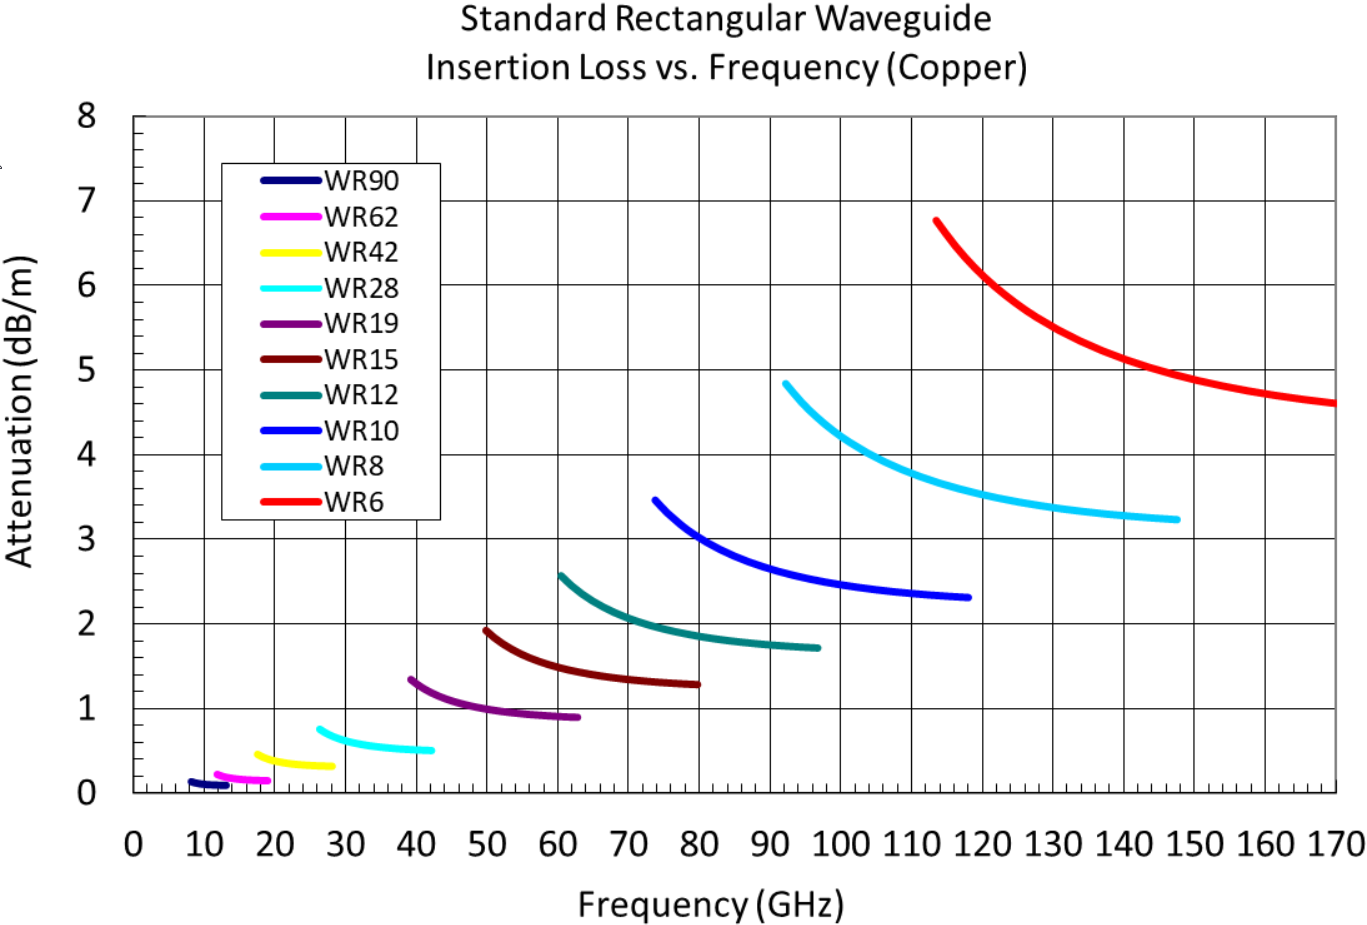
\includegraphics[width=0.6\linewidth]{waveguides}
	\label{fig:waveguides}
	\caption{Waveguides offer much lower losses (and the Y--axis scale is in dB per METER).
	The highest loses are for waveguide WR6, which is around \textbf{7 dB/m = 0.07 dB/cm}.
	In terms of total losses, the microstrips and striplines cannot compete with the waveguides.}
	(image source: https://sagemillimeter.com)
\end{figure}

\section{Summary}
That lead to a very important conclusion -- the software for simulation has its limitations and it's much appreciated to use different tools (PCAAD, MicrowaveStudio, $\mu$Wave Wizard etc.).\\
Additionally, as it was told in the classes during the tour in the Microwave Laboratory, the professional tools are very expensive, but they also deliver the quality tools that cannot be compared to the ones available in the internet. 
\\
\\
In terms of total losses in the different medium, the waveguides are incomparable in terms of their quality. Unfortunately, they are much bigger in terms of their physical dimensions and much more expensive in comparison to the microstrip/striplines.\\
Also their operating frequencies are much higher than microstrip/stripline can deal with -- at it was observed in the results from the table, the losses at 1GHz are significant, not to mention the calculation result in case of 20GHz. But the waveguids can deal with these frequencies very effectively.

\chapter{Impedance transformation}
\section{Problem statement}
Taking the presented below model, the input impedance should be calculated according to correct formulas.\\
The presented list of values should be use in these calculations as follows:
R1 [0, 50, 70] $\Omega$,\\
R2 [0, 25, 50, 70]$\Omega$,\\
L0 $<$5, 200$>$mm with 25mm step,\\
L1 [13, 42, 72]mm\\
L2 [25, 42, 93]mm\\
\begin{figure}[h]
	\centering
	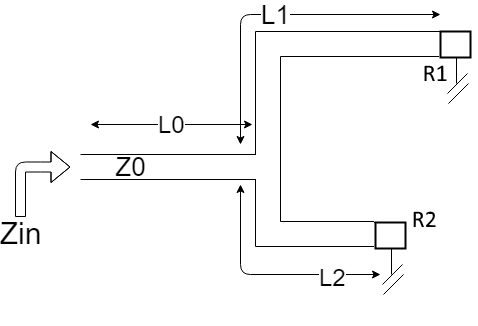
\includegraphics[width=0.4\linewidth]{impedance}
	\label{fig:impedance}
	\caption{The model of junction to be used in input impedance calculation.}
\end{figure}

If any other parameter will be necessary, there should be assumed that they are constant as follows:\\
$f_0$ = 5 GHz\\
$\epsilon _r$ = 2.3,\\  tan$\delta$ = 0.001, \\laminate\_thickness = 0.508mm, \\copper\_thickness = 18$\mu$m
\\
\\
\section{Task realization}
By utilizing the presented during classes equations, the impedance was calculated.\\
\begin{align*}
Z' &= \frac{Z_1 ' Z_2 '}{Z_1 ' + Z_2 '}\\
\\
Z_{in} &= Z_0 \frac{Z_L + jZ_0tan(\beta L)}{Z_0 + jZ_Ltan(\beta L)}
\end{align*}

\noindent
With the given data almost 1000 results were obtained (there was dedicated software script prepared in the Python language to calculate the impedance and automatically save the results as Excel file).
\\
To maintain the clean view in the report, only the part of the results will be presented in tabular form (as the examples). The most meaningful will be the prepared plots.

\begin{table}[h]
	\centering
	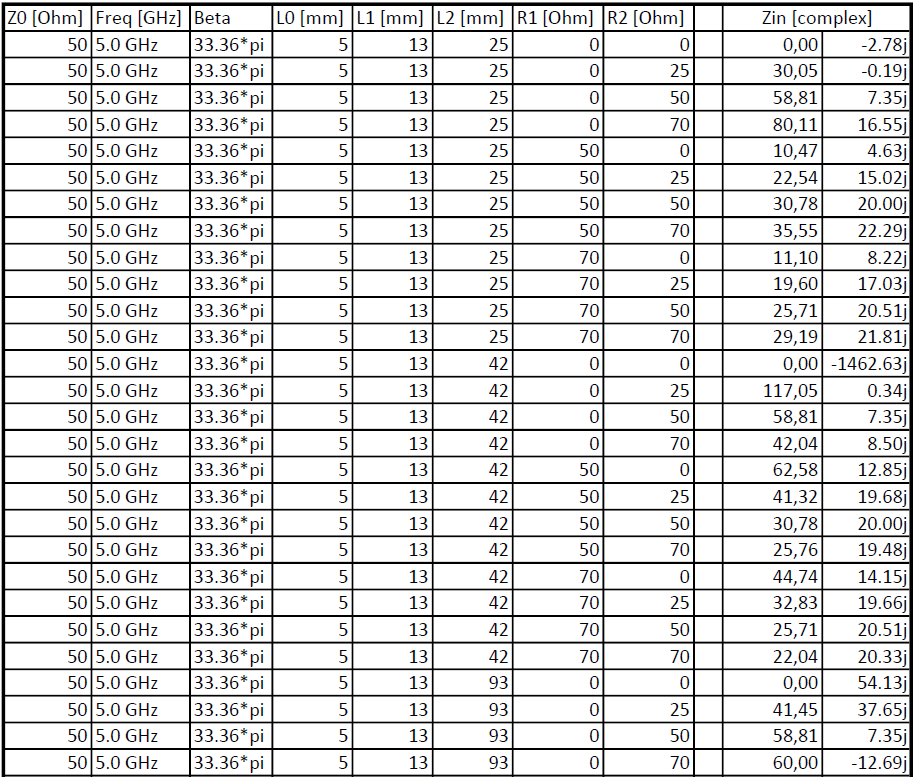
\includegraphics[width=0.7\linewidth]{microwave-fail1}
	\caption{The input impedance (Zin) calculated based on the presented model and given formulas. Although the realation between parameters cannot be establish based only on numerical results, some observations can be made. It can be observed, that in cases when the R1 and R2 resistances are equal to zero, the input impedance consist only the imaginary part of complex number and the real part is equal to zero.}
	\label{fig:microwave-fail1}
\end{table}
\newpage
\begin{figure}[!h]
	\centering
	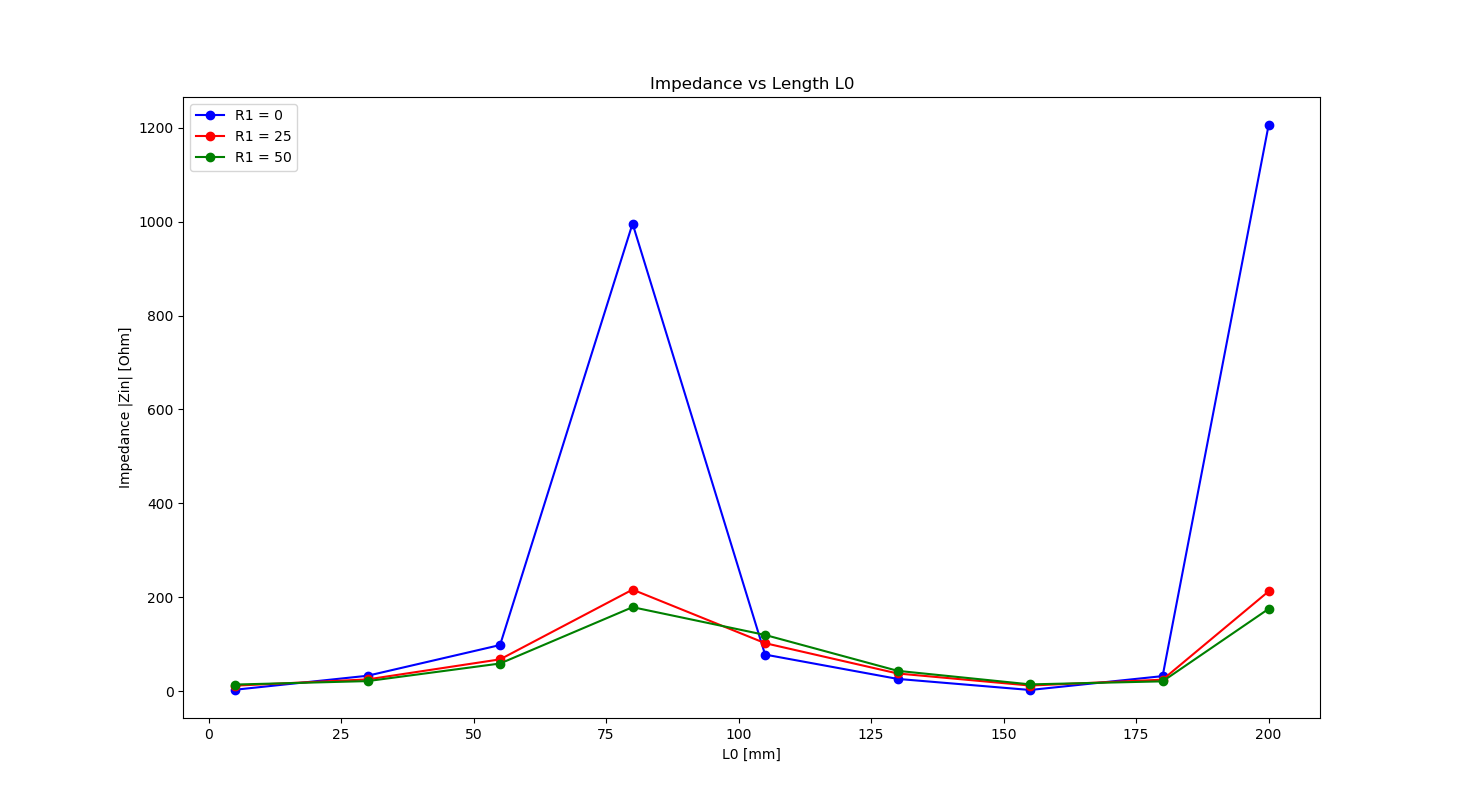
\includegraphics[width=1\linewidth]{Figure_4}
	L1 == 13mm, L2 == 25mm, R2 == 0 Ohm
	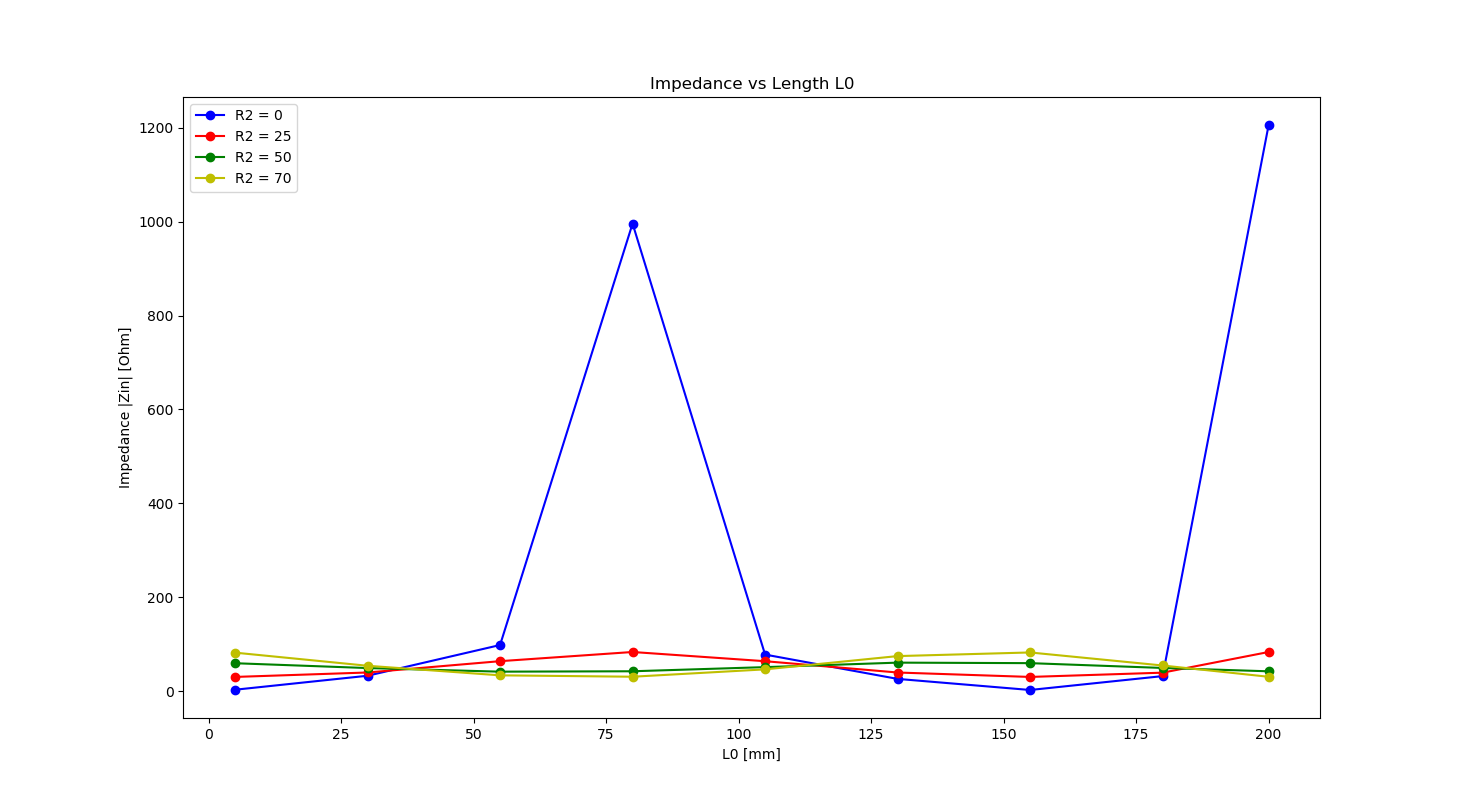
\includegraphics[width=1\linewidth]{Figure_5}
	L2 == 13mm, L1 == 25mm, R1 == 0 Ohm
	\caption{The impedance magnitude versus length L0. The family of curves is related to different values of R1 and R2.\\
	The relation between length and impedance can be observed -- it seems that there is periodical plot with some minimum and maximum value at certain lengths. The bigger the resistances R1 and R2, the smaller the deviation of the input impedance. It reaches the maximum for the case where R1/R2 are equal to zero (the circuit load is 0 at one or second end).
	}
\end{figure}

\begin{figure}[!h]
	\centering
	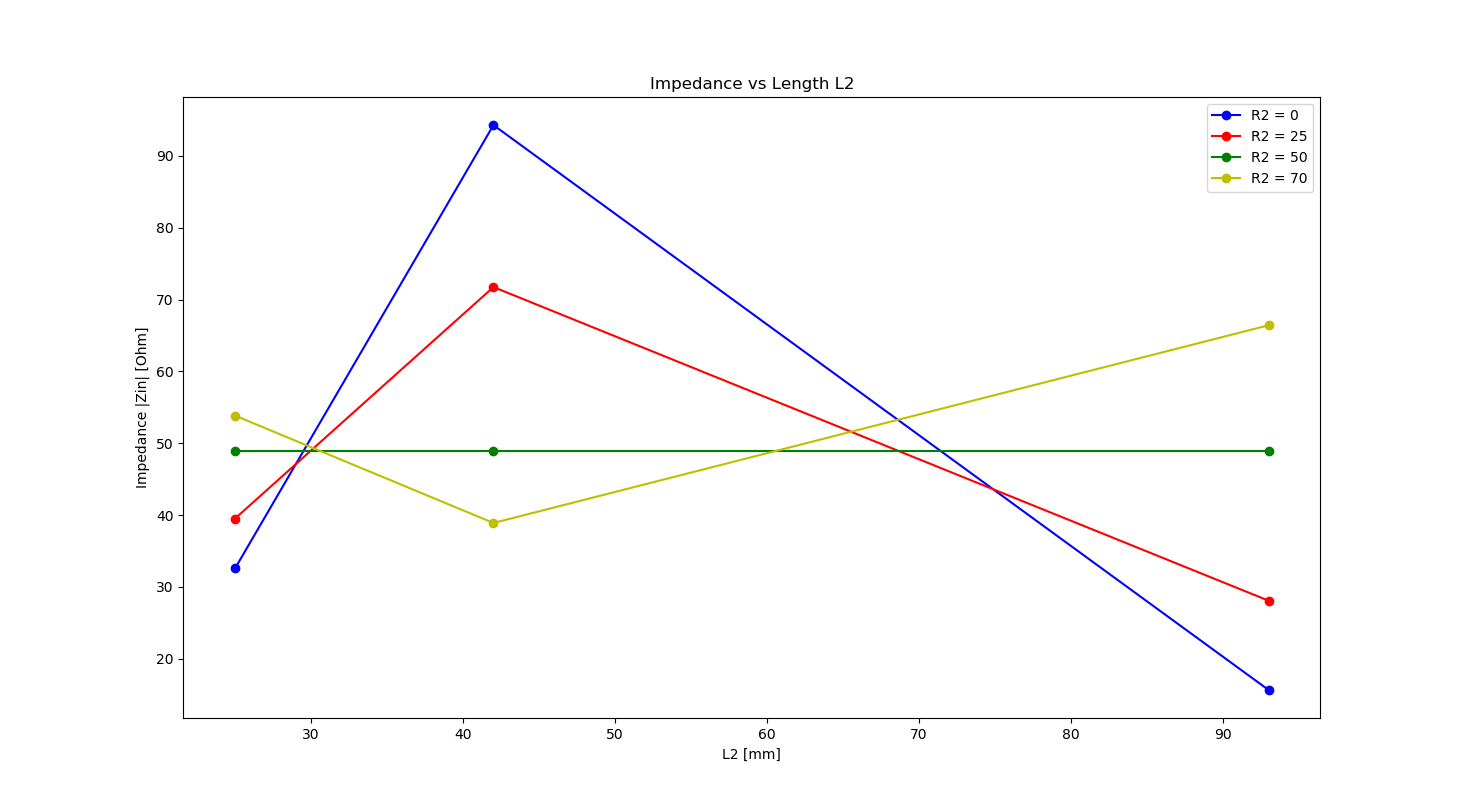
\includegraphics[width=1\linewidth]{Figure_3}
	L0 = 30mm, L1 == 13mm, R1 = 0 Ohm
	\caption{The picture presents the magnitude of impedance in relation to length L2. With changing length the impedance seems to change alternately between maximum and minimum value. However, there is a line for R2 = 50 Ohm, which is completely flat. At this point it seems, that for some value of load, the length of path simply does not take an effect.}
		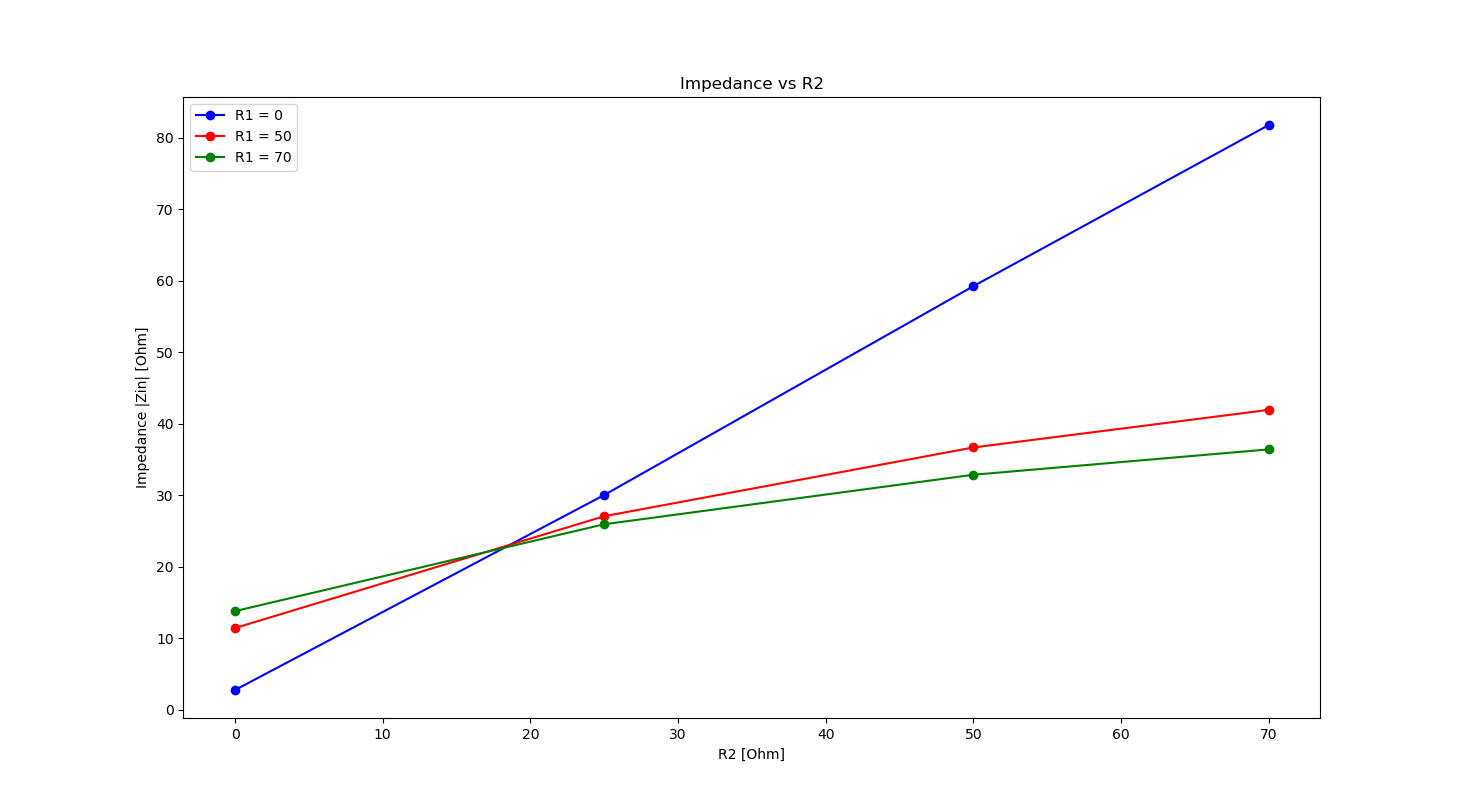
\includegraphics[width=1\linewidth]{Figure_1}
	L0 == 30mm, L1 == 13mm, L2 == 25mm,
	\caption{Relation between R2 (x-axis), R1 (curves family) and magnitude of impedance Zin. For lengths taken as constant, we can observe that in selected ranges, the increasing values of R2 resulted in greater magnitude of impedance. Also the curves family of R1 changes its angle of elevation to X--axis, that results in much steep plot.}
\end{figure}


\begin{figure}[!h]
	\centering
	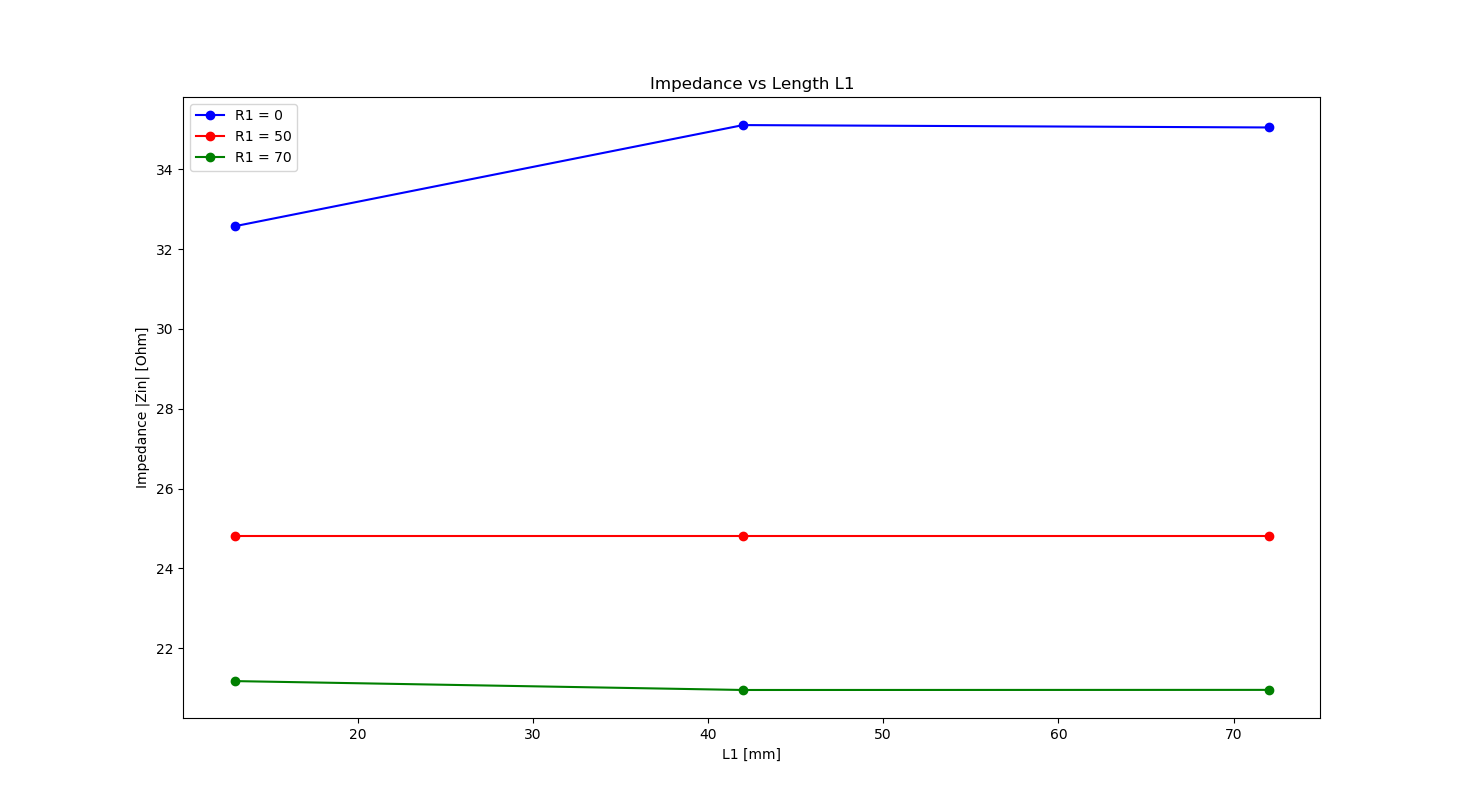
\includegraphics[width=1\linewidth]{Figure_2}
	L0 == 30mm, L2 == 25mm
	\caption{As there are only three selected values of L1, this plot may not be very informative in particular. However, the relation between Zin and L1 (also with related curves family of R1), can inform us that the influence of L1 (no matter the load at its end) is not very significant.}
\end{figure}

\section{Summary}
In this assignment the numerous cases within given ranges of values were calculated. The task was to calculate it and try to find the relation between data and input impedance.\\
The two formulas are not very complicated, but the analysis of results requires more than just table with numerical results. That was the case for preparing the plots.\\
\\
Based on presented plots, some relationships between data were established. There were periodical dependencies (seems that it was related to the phase in different lengths), some parameters that had very small influence, but also clear conclusions (just like in the last presented picture).
Nevertheless, it is much clearer to discuss results having the plots that can be referred to. It is more informative way to discuss observed aspects of physical phenomena.

\chapter{Fractional--n PLL with VCO}
\section{Problem statement}
The given assignment purpose was to read the HMC778 documentation guide and prepare in short the understanding of fractional--N PLL circuit.\\
By documentation sheet further investigation, the design of the PCB should be described in order to achieve the best possible performance.
\section{Task Realization}
\begin{figure}[!h]
	\centering
	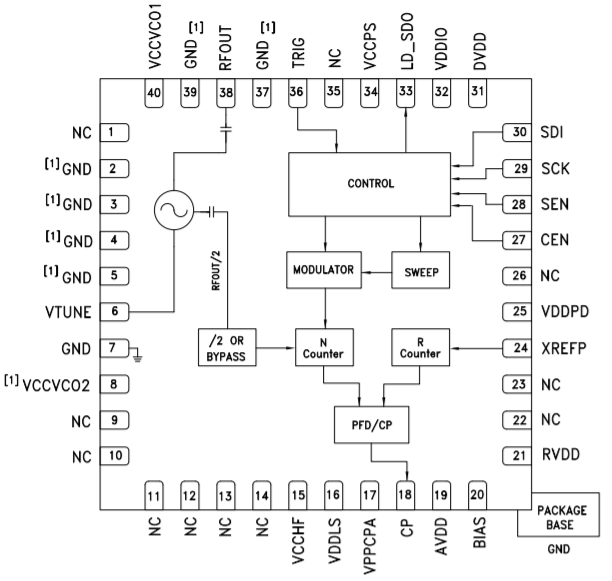
\includegraphics[width=0.5\linewidth]{pll}
	\label{fig:pll}
	\caption{Functional diagram of the selected PLL circuit chip.}
	
	(source: "PLLs with integrated VCO - Microwave Applications
	product \& operating guide", Analog Devices)
\end{figure}
\noindent
\subsubsection{Circuit information}
The HMC778LP6CE is a fully functioned Fractional-N Phase-Locked-Loop (PLL) Frequency Synthesizer with an
integrated Voltage Controlled Oscillator (VCO). \\
The official datasheet is describing the input reference frequency range to be DC to 350 MHz. The manufacturer claims that it provide very good phase noise performance over temperature,
shock and process. The HMC778LP6CE offers frequency sweep and modulation features, external triggering, double-buffering, exact frequency control, phase modulation.\\ \\ The HMC778LP6CE is packaged
in a leadless QFN 6 x 6 mm surface mount package.

\subsubsection{PLL operation}
The assignment was to prepare a short summary of principles of PLLs operation of the HMC778 circuit and to describe the difference in operation between integer and fractional PLLs.
\\
The basic application of PLL integrated circuit such as HMC778 is to form a control loop to multiply low frequency source to a higher frequency.

\begin{figure}[!h]
{	
	\centering 	
	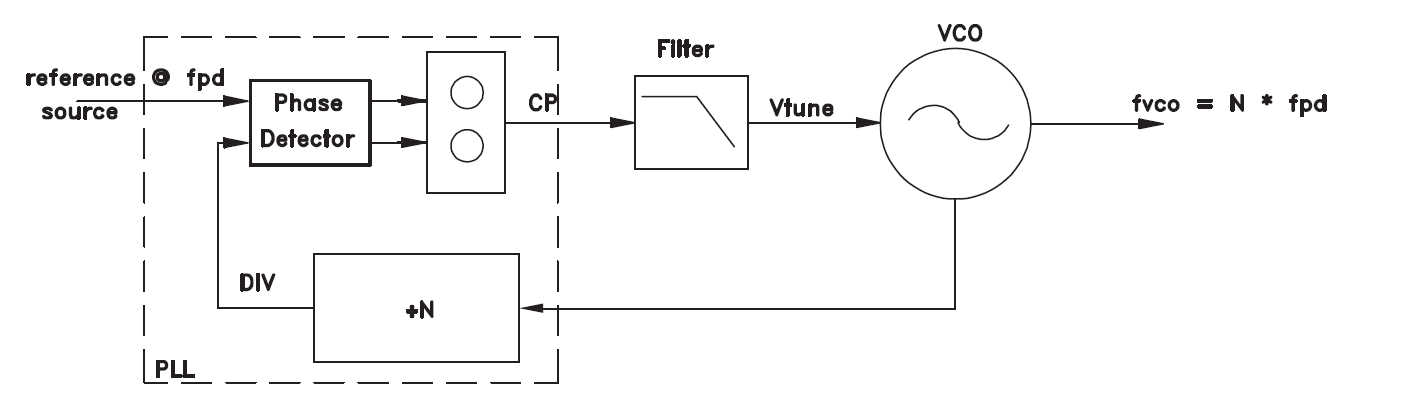
\includegraphics[width=1\linewidth]{pll3}}
	\caption{The phase detector and charge--pump drive the tuning signal of VCO (voltage controlled oscillator) to bring the phases (phases of both reference signal and tuning signal) at the detector input into alignment.\\
	If the loop succeeds, then the phase detector inputs (reference and DIV at the diagram) are at the same frequency. 
	As the frequency of DIV = $f_{VCO} / N$, then its equality means that control loop forced the frequency of VCO to be N $\cdot f_{PD}$.}
	\hspace{20pt}

	(image source: "PLLs with integrated VCO - Microwave Applications
	product \& operating guide", Analog Devices)
\label{fig:pll3}
\end{figure}
\vspace{20pt}
The difference between integer and fractional PLL is that the fractional can bring N value at fractional level (1.6, 2.4, 3.7) while the integer can do it only with discrete value of N (2, 4, 10, 13 etc.).

\newpage
\subsubsection{Designing PCB for HMC778}
\begin{figure}[!h]
	\centering
	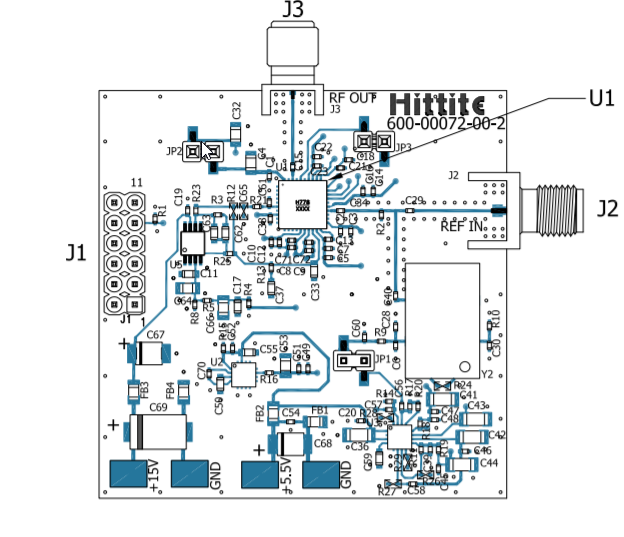
\includegraphics[width=0.5\linewidth]{pll2}
	\label{fig:pll2}
	\caption{Example usage of HMC778 chip -- an evaluation board that follows the guidelines in the PCB design.}
	\hspace{20pt}
	(image source: "PLLs with integrated VCO - Microwave Applications
	product \& operating guide", Analog Devices)
\end{figure}
Guidelines to design a PCB board to be utilized in the future:
\begin{itemize}
	\item The circuit board used in the application should use RF circuit design techniques. 
	\item Signal lines should have
	50 Ohm impedance while the package ground leads and exposed paddle should be connected directly
	to the ground plane. 
	\item A sufficient number of via holes should be used to connect the
	top and bottom ground planes.
\end{itemize}
\section{Summary}
The HMC778 chip is a fractional-N pll (Phased--Lock--Loop) -- the applications of this type of chips is to build a control loop to multiply low frequency source to a higher frequencies.\\
The difference between integer and fractional PLL is that the fractional can bring N value at fractional level, while the integer can do it only with discrete value of N (2, 4, 10, 13).\\
\\
\\
Beside of having the selected chip, it should also be assembled into the PCB board. It is a very sensitive element, therefore it requires proper design of the circuit board.\\ The chip's official documentation contains relevant examples and informations that should be followed when designing either prototype or final product.

\chapter{Free--space path losses}
\section{Problem statement}
During the laboratory, the aspect of free--space losses and started the evaluation according to the distance was discussed. This task was to finish the calculations that started during the classes and prepared the comparison in the tabular form.

\section{Task realization}
The losses were calculated with "Free--Space Path Loss Calculator" from \textbf{Pasternack website}.
\begin{figure}[h]
	\centering
	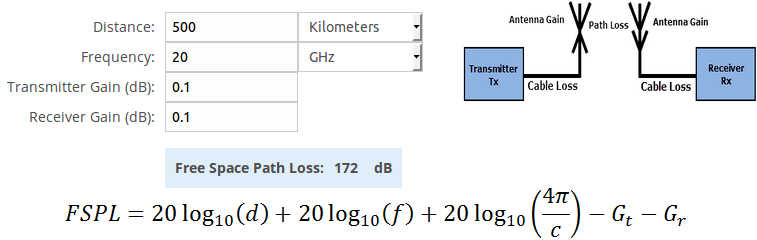
\includegraphics[width=0.6\linewidth]{pasternack}
	\caption{Free--space loss calculator by https://www.pasternack.com/}
\end{figure}

\begin{table}[h]
	\centering
	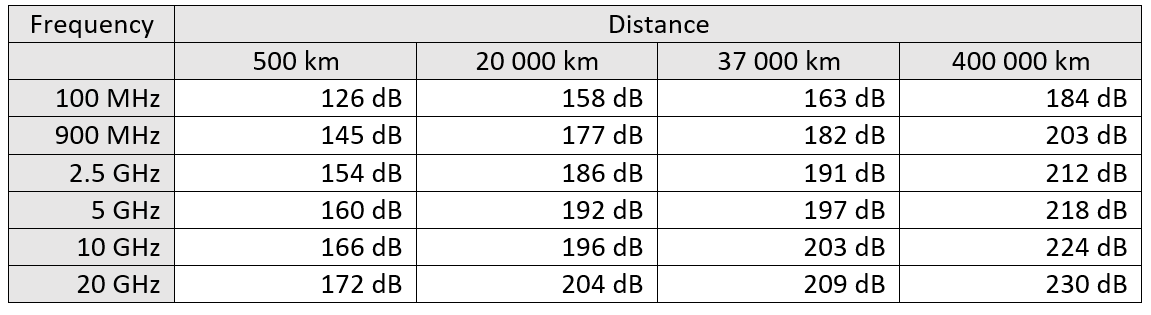
\includegraphics[width=0.9\linewidth]{freespace}
	\caption{The comparison of free--space losses in relation to used frequency and distance between transmitter and receiver. It is clear that losses increase when the higher frequencies are used or the distance is larger.}
	\label{fig:freespace}
\end{table}

To deliver also the visual representation of the obtained results, the plot (with family of curves for distances) was prepared.\\
It delivers exactly the same information, however the conclusions can be seen instantly.
\begin{figure}[h]
\centering
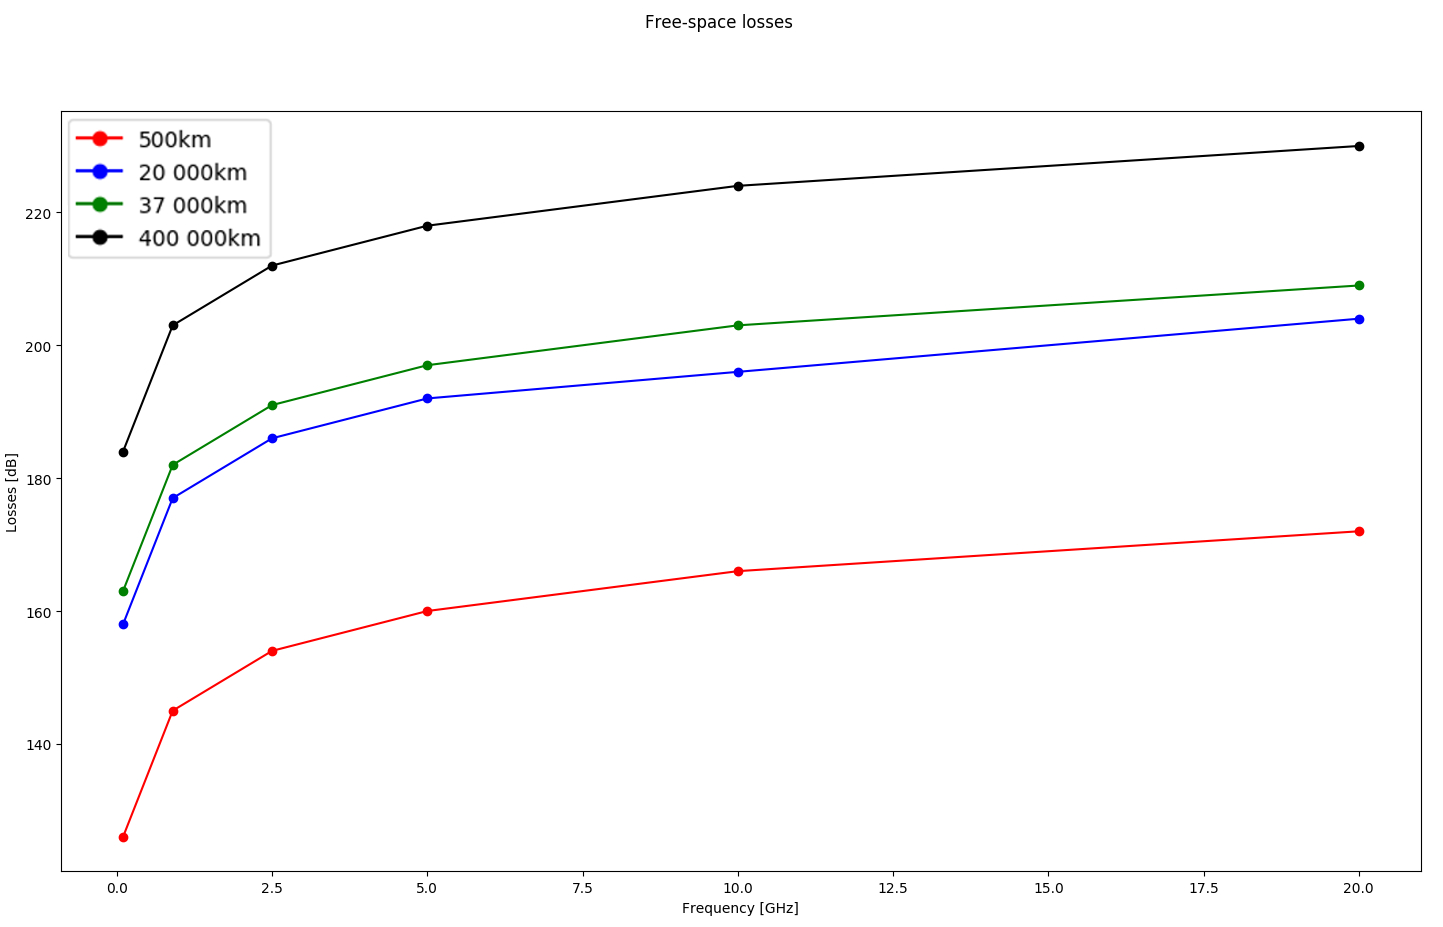
\includegraphics[width=1\linewidth]{freespaceloss}
\caption{Calculated free--space losses presented as a plot. The data is exactly the same as used in the tabular form.}
\label{fig:freespaceloss}
\end{figure}

\noindent
\section{Summary}
The table observation leads to a clear ans simple conclusion -- the free--space losses are increasing when using higher frequencies. They also increase with the distance, what is a common behavior due to energy dispersion along the distance.
\newpage
\chapter{Microwave low--noise amplifier operating at C--band}
\section{Problem statement}
The goal of the following assignment is to choose a low--noise amplifier that is operating at C--band (it was recommended to amplifiers from Qorvo company). The investigation over the amplifier's technical specification should be done as well as  simulation prepared e.g. in Ansoft Designer software (based on scattering matrix data).
\section{Task realization}
\subsubsection{Choosing the amplifier}
The C--band is a portion of the electromagnetic spectrum in the microwave range of frequencies ranging from 4.0 to 8.0 GHz (according to IEEE designation).\\
To fulfill the given assignment, the packed low noise amplifier manufactured by Qorvo was chosen. It is \textbf{TGA2611--SM} model, operating at frequency range 2.0 - 6.0 GHz, so its range of operation covers C--band.
\\
It is said, that the product is designed to commercial and military radars or communication.\\
Its noise figure is estimated to be 1.0 dB.

\begin{figure}[h]
	\centering
	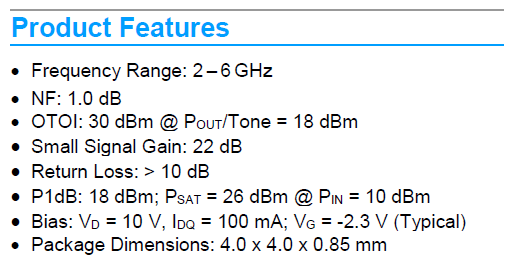
\includegraphics[width=0.5\linewidth]{chip}
	\caption{Basic features of selected amplifier TGA2611--SM.}
	(source: TGA2611-SM 2 - 6 GHz GaN Low Noise Amplifier Datasheet, Qorvo)
	\label{fig:chip}
\end{figure}
%The *.s2p file describing the scattering matrix of the plot was obtained from the Qorvo site. In the Ansoft Designer there was prepared a report:
\subsubsection{Scattering matrix analysis}
\begin{figure}[!h]
	\centering
	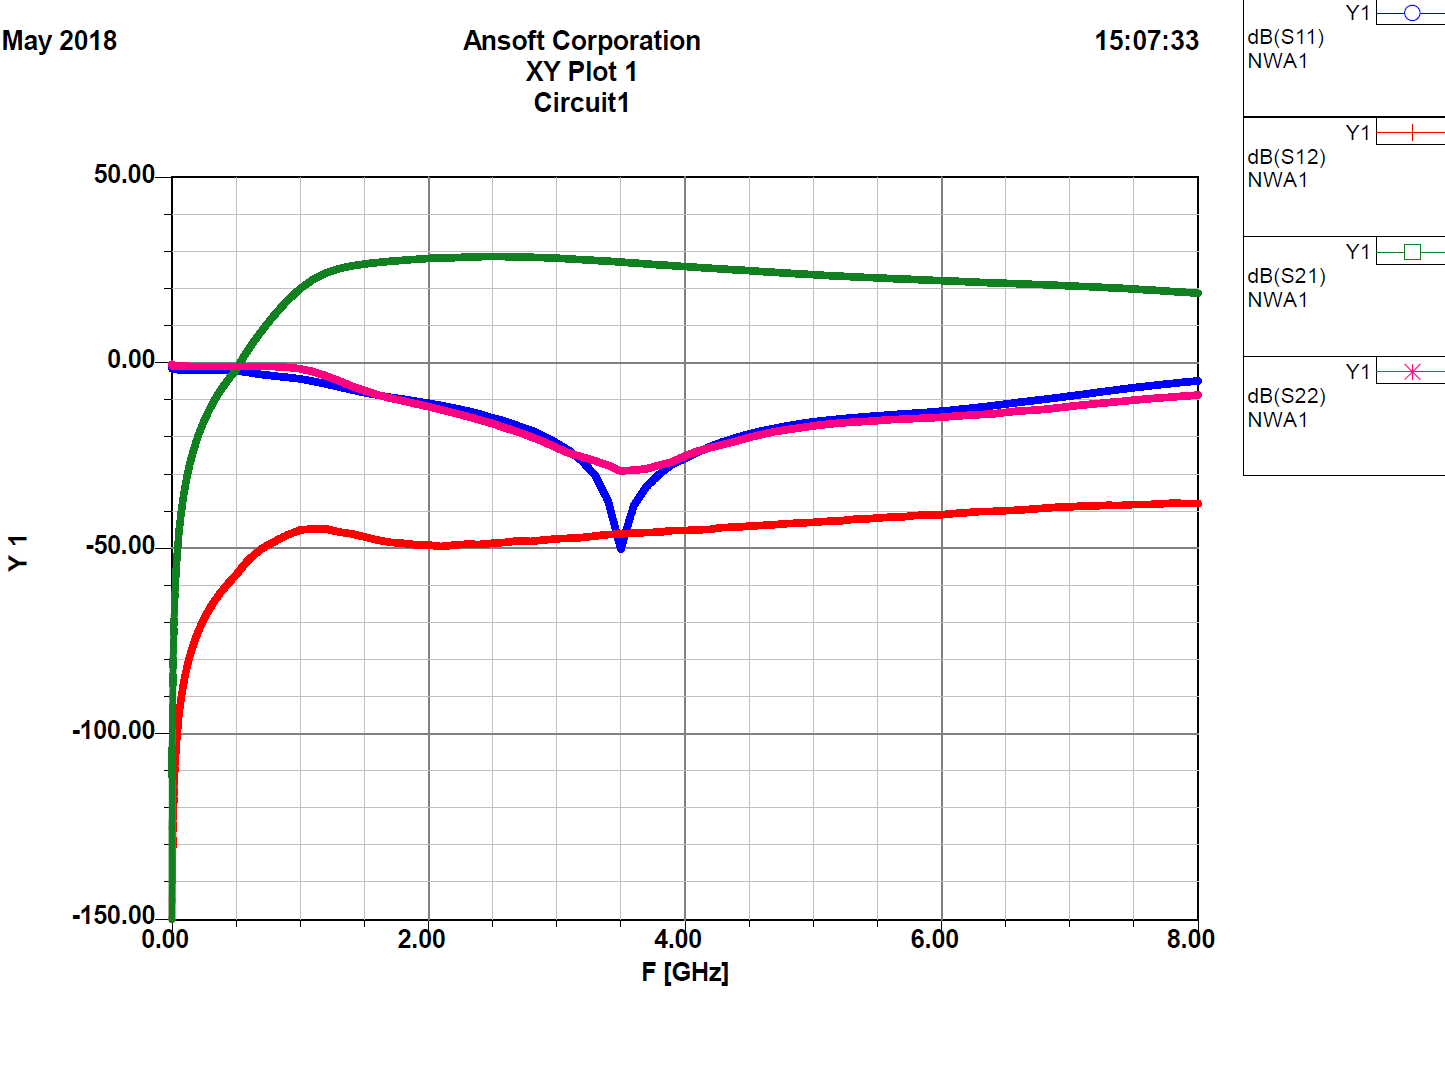
\includegraphics[width=0.7\linewidth]{chip-plot}
	
	(Scattering matrix plots generated in Ansoft Designer)
	
	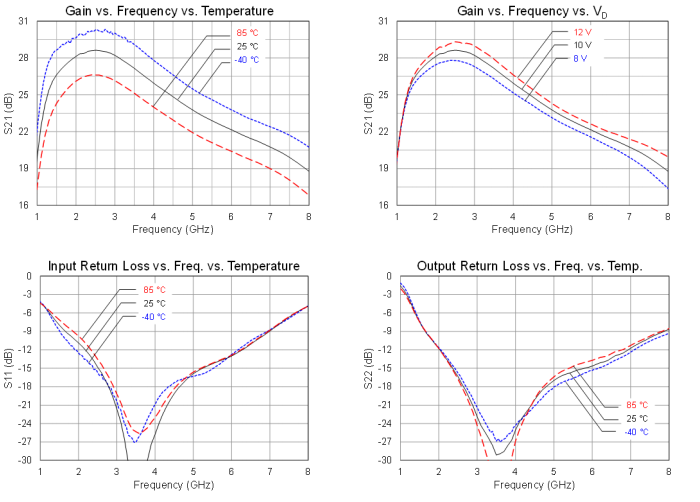
\includegraphics[width=0.7\linewidth]{amplifier}
	
	(source: TGA2611-SM 2 - 6 GHz GaN Low Noise Amplifier Datasheet, Qorvo)

	\caption{Plot of the scattering matrix prepared in Ansoft Designer, based on *.s2p file. The four plots are taken from the datasheet for comparison. By observing the plots it can be noticed, that the scattering matrix parameters values are very similar to each other in both cases. The documentation of course includes also the plots at different temperatures, but the ranges of values seems to be correct.}
	\label{fig:chip-plot}
\end{figure}
The Scattering matrix describes the following aspects of the N--port element:
\begin{itemize}\setlength\itemsep{1pt}
\item S11 input return loss  (blue plot)
\item S12 reverse gain       (red plot)
\item S21 small signal gain  (green plot)
\item S22 output return loss (pink plot)
\end{itemize}
\newpage
\subsubsection{Application Circuit}
\begin{figure}[h]
	\centering
	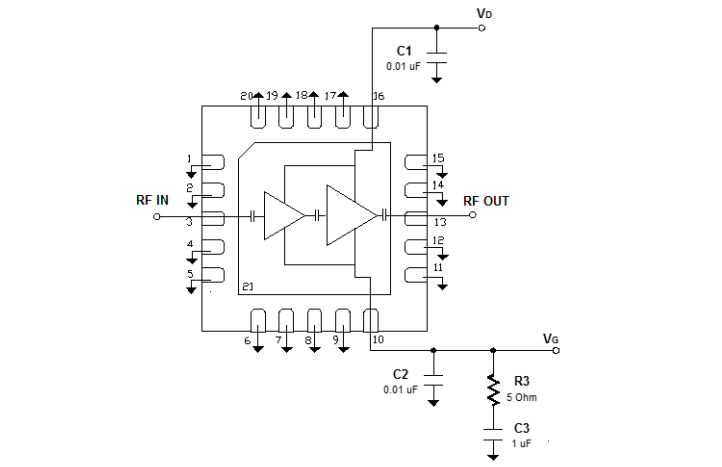
\includegraphics[width=0.7\linewidth]{amplifier1}
	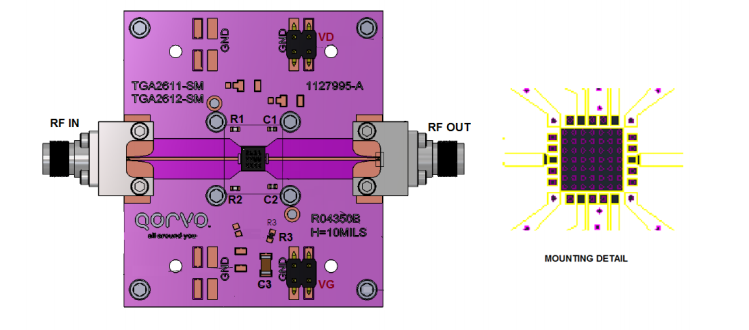
\includegraphics[width=0.7\linewidth]{amplifier2}
	\caption{Application circuit example delivered by Qorvo. The circuit requires additional electrical elements at $V_d$ and $V_g$.\\
	As the element in Ansoft Designer was declared as N--port element defined by *.s2p file (so it was two--port), there was no possibility to simulate the application circuit.}\vspace{20pt}	(image source: TGA2611-SM 2 - 6 GHz GaN Low Noise Amplifier Datasheet, Qorvo)
	\label{fig:amplifier1}
\end{figure}

The Qorvo company delivered also some information and guidelines for designing application circuit:
\begin{itemize}
\item The microstrip line at the connector interface is optimized for the Southwest Microwave end launch connector 1092-01A-5.
\item The pad pattern shown has been developed and tested for optimized assembly at Qorvo. 
\item The PCB land pattern has been
developed to accommodate lead tolerances. Since processes vary from company to company, careful process development
is recommended.
\item Multiple vias should be employed under the package center paddle to minimize inductance resistance.
\end{itemize}


\subsubsection{Noise Figure}
The plot below presents the noise figure of the selected amplifier.
\begin{figure}[h]
	\centering
	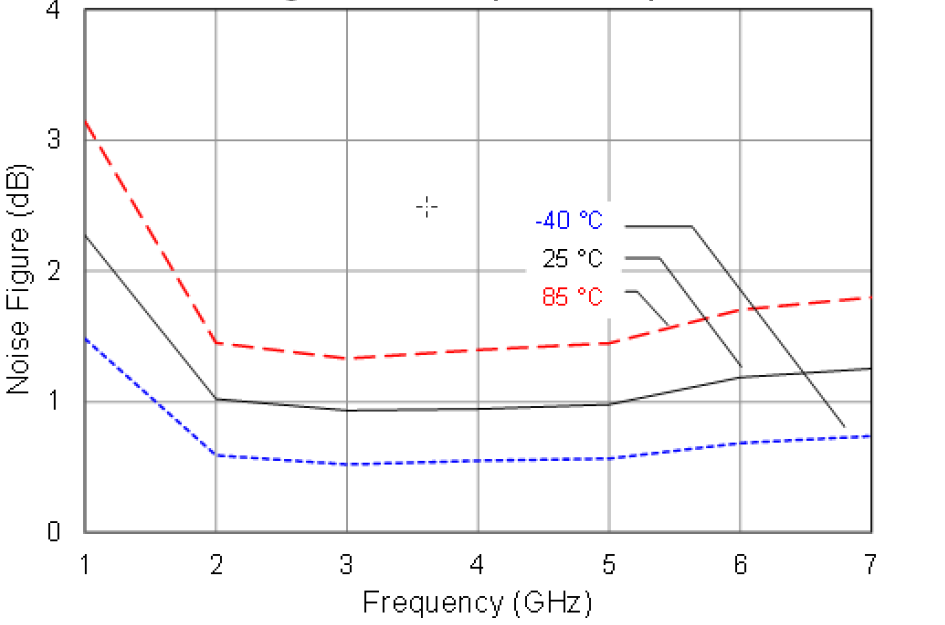
\includegraphics[width=0.6\linewidth]{noise}
	\caption{Noise figure vs frequency (at different temperatures).}
	(source: TGA2611-SM 2 - 6 GHz GaN Low Noise Amplifier Datasheet, Qorvo)
	\label{fig:noise}
\end{figure}

Despite advertised 1dB noise figure in the operating range (reminder: 2 -- 6 GHz), when approaching the upper limit of 6 GHz the NF increases. However, the change is very insignificant (more or less it is 1.25 dB).\\
Of course also the temperature is important, but also at 85 $^\circ$C
the NF in operating range is around 1.75 dB.

\section{Summary}
The microwave equipement needs to be carefully chosen and the final solution (PCB board) designed according to microwave engineering rules. When operating at high frequency, even the smallest differences in fabrication can have significant impact on the performance. The producer also proposes some guidelines in PCB fabrication with notice that careful developement process is recommended.\\
It is very important to read the technical documentation and investigate all data that is delivered by producer. The tables with parameters on the websites are purely for marketing business and often the best parameters are listed. The technical documentation delivers much more detailed specification.\\
\\
The choice of professional tools is significant aspect of designing microwave engineering solution. \textbf{Ansoft Designer} is one of many available tools, but in comparison to \textbf{CST MICROWAVE STUDIO 3D EM Simulation Software} (it was presented during the tour in the Antenna Laboratory at Wroclaw Unicersity of Science and Technology) has very limited options of usage.
\begin{thebibliography}{9}
\bibitem{microwave} Online Microwave Encyclopedia, http://microwave101.com,  (27.02.2018)
\end{thebibliography}
\end{document}